\documentclass{article}

\usepackage{pandekten}
\usepackage{dashrule}

\makeatletter
\newcommand*{\shifttext}[1]{%
  \settowidth{\@tempdima}{#1}%
  \hspace{-\@tempdima}#1%
}
\newcommand{\plabel}[1]{%
\shifttext{\textbf{#1}\quad}%
}
\newcommand{\prule}{%
\begin{center}%
\hdashrule[0.5ex]{.99\linewidth}{1pt}{1pt 2.5pt}%
\end{center}%
}

\makeatother

\newcommand{\minusbaseline}{\abovedisplayskip=0pt\abovedisplayshortskip=0pt~\vspace*{-\baselineskip}}%

\setlength{\parindent}{0pt}

\title{Assignment 7}
\author{Ze Chen}

\begin{document}

\maketitle

\plabel{1}
The Feynman rules are listed below.
\begin{itemize}
    \item External leg contractions:
    \begin{center}
        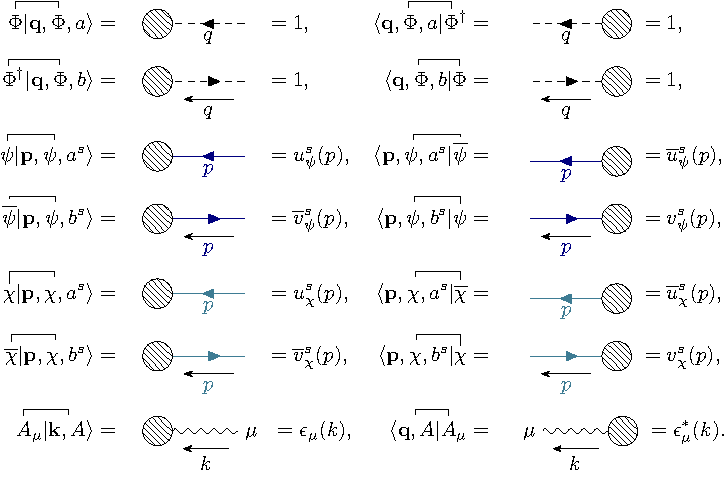
\includegraphics{img/leg/leg.pdf}
    \end{center}
    \item Vertices:
    \begin{center}
        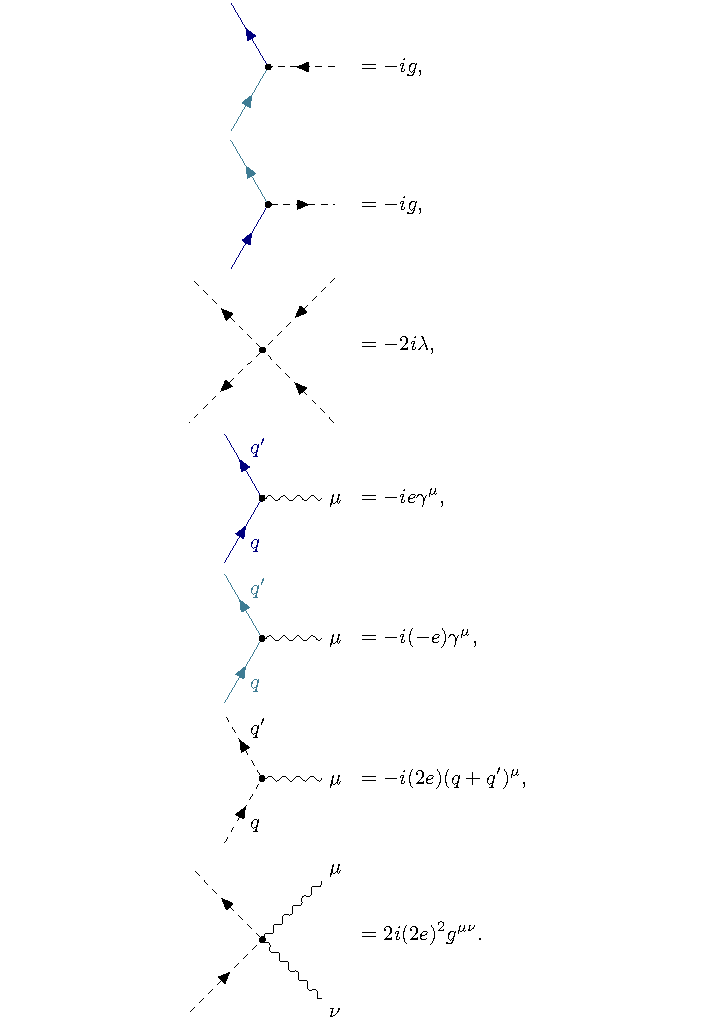
\includegraphics{img/vertex/vertex.pdf}
    \end{center}
    \item Propagators:
    \begin{center}
        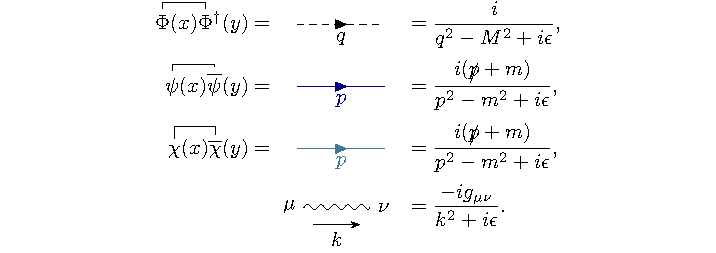
\includegraphics{img/propagator/propagator.pdf}
    \end{center}
\end{itemize}

% \bibliographystyle{plain}
% \bibliography{main}

\plabel{(a)}%
The equations of motion are given by
\begin{align*}
    \partial^2 \Phi + M^2 \Phi + g\overline{\chi} \psi &= 0, \\
    -i\slashed{\partial} \psi + m\psi + g\Phi\chi &= 0, \\
    -i\slashed{\partial} \chi + m\chi + g\Phi^\dagger \psi &= 0.
\end{align*}
The transformation $\psi \rightarrow e^{i\alpha}\psi$, $\chi \rightarrow e^{i\beta}\chi$, and $\Phi \rightarrow e^{i(\alpha - \beta)} \Phi$ gives
\[ j^\mu_\psi = i\qty[(\partial^\mu \Phi^\dagger)\Phi - \Phi^\dagger \partial^\mu \Phi] + \overline{\psi} \gamma^\mu \psi \]
and
\[ j^\mu_\chi = -i\qty[(\partial^\mu \Phi^\dagger)\Phi - \Phi^\dagger \partial^\mu \Phi] + \overline{\chi} \gamma^\mu \chi. \]

Even if $m=0$ the axial currents may not be conserved unless $g=0$, in which case
\[ j^\mu_\psi = \overline{\psi} \gamma^\mu \qty(\frac{1\pm \gamma^5}{2}) \psi \]
and
\[ j^\mu_\chi = \overline{\chi} \gamma^\mu \qty(\frac{1\pm \gamma^5}{2}) \chi. \]

Translation and rotation symmetry gives the energy-momentum tensor and angular momentum respectively.

\plabel{(b)}%
The leading order of decay is given by the following diagram.
\begin{center}
    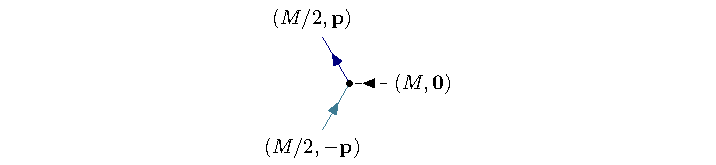
\includegraphics{img/decay/decay.pdf}
\end{center}
We find
\[ \abs{\mathcal{M}}^2 = g^2 \sum_{r,s} \overline{v}^r(M/2,\vb{p}) {u}^s(M/2,-\vb{p})\overline{u}^s(M/2,-\vb{p}) {v}^r(M/2,\vb{p}) = 8 g^2 \abs{\vb{p}}^2. \]
With the result from problem 2 of assignment 5 we find
\[ \Gamma = \frac{\abs{\vb{p}}}{8\pi M^2} \abs{\mathcal{M}}^2 = \frac{g^2}{8\pi M^2}\qty(M^2 - 4m^2)^{3/2} \]
since
\[ \vb{p} = \frac{\sqrt{M^2 - 4m^2}}{2}. \]

\plabel{(c)}%
The interaction is given by
\[ S = \int \dd[4]{x} \qty{ -e \overline{\psi}\gamma^\mu \psi A_\mu + e \overline{\chi}\gamma^\mu \chi A_\mu - 2ie A^\mu\qty[\Phi^\dagger(\partial_\mu \Phi) - (\partial_\mu \Phi^\dagger)\Phi] + 4e^2 A^\mu A_\mu \Phi^\dagger \Phi }. \]
The diagram through $\Phi$ is given below.
\begin{center}
    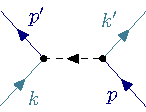
\includegraphics{img/scatter/scalar.pdf}
\end{center}
Let $u = p - k'$.
Then this diagram gives
\[ i\mathcal{M} = -ig^2 \frac{\qty(\overline{u}(p') u(k))\qty(\overline{u}(k')u(p))}{u^2 - M^2}. \]
The diagram through photon is given below.
\begin{center}
    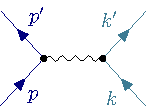
\includegraphics{img/scatter/photon.pdf}
\end{center}
Let $t = p-p'$.
Then this diagram gives
\[ i\mathcal{M} = -ie^2 \frac{\qty(\overline{u}(p')\gamma^\mu u(p))\qty(\overline{u}(k')\gamma_\mu u(k))}{t^2}. \]
Let $\vb{p}\cdot \vb{p}' = \abs{\vb{p}}^2 \cos\theta$ and $E = \sqrt{m^2+\abs{\vb{p}}^2}$.
To obtain the total $\abs{\mathcal{M}}^2$, note that
\begin{align*}
    &\phantom{{}={}} \frac{1}{4} \sum_{\text{spins}} \qty[\qty(\overline{u}(p') u(k))\qty(\overline{u}(k')u(p))]\qty[\qty(\overline{u}(p') u(k))\qty(\overline{u}(k')u(p))]^* \\
    &= 4(k\cdot p' + m^2)(k'\cdot p + m^2) \\
    &= 4(E^2 + (E^2 - m^2) \cos\theta + m^2)^2, \\
    &\phantom{{}={}} \frac{1}{4} \sum_{\text{spins}} \qty[\qty(\overline{u}(p') u(k))\qty(\overline{u}(k')u(p))] \qty[\qty(\overline{u}(p')\gamma^\mu u(p))\qty(\overline{u}(k')\gamma_\mu u(k))]^* \\
    &= -2m^2(k'\cdot p' + k\cdot k' + k \cdot p + p\cdot p') + 4m^2(p\cdot k' + k\cdot p') + 4(k\cdot p')(p\cdot k') + 4m^2 \\
    &= 4 \left(E^4-E^2 m^2+( \cos \theta ) \left(2 E^4+\left(E^2-m^2\right)^2 ( \cos \theta )+E^2 m^2-3 m^4\right)+2 m^4\right), \\
    &\phantom{{}={}} \frac{1}{4} \sum_{\text{spins}} \qty[\qty(\overline{u}(p')\gamma^\mu u(p))\qty(\overline{u}(k')\gamma_\mu u(k))]\qty[\qty(\overline{u}(p')\gamma^\mu u(p))\qty(\overline{u}(k')\gamma_\mu u(k))]^* \\
    &= 8\qty[-m^2 (k\cdot k') + (k\cdot p')(p\cdot k') +(k\cdot p)(k'\cdot p') - m^2 (p\cdot p') + 2m^4] \\
    &= 8 \left(2 \left(E^4-m^4\right) (\cos \theta  )+5 E^4+\left(E^2-m^2\right)^2 \left(\cos ^2 \theta  \right)-6 E^2 m^2+3 m^4\right).
\end{align*}
Therefore,
\begin{align*}
    &\phantom{{}={}} \frac{1}{4} \sum_{\text{spins}} \abs{\mathcal{M}}^2 \\
    &= g^4 \frac{4(E^2 + (E^2 - m^2) \cos\theta + m^2)^2}{\qty[2(E^2 - m^2)(1+\cos\theta) + M^2]^2} \\
    &\phantom{{}={}} + g^2 e^2 \frac{8 \left(E^4-E^2 m^2+( \cos \theta ) \left(2 E^4+\left(E^2-m^2\right)^2 ( \cos \theta )+E^2 m^2-3 m^4\right)+2 m^4\right)}{\qty[2(E^2 - m^2)(1+\cos\theta) + M^2]\qty[2(E^2-m^2)(1-\cos\theta)]} \\
    &{\phantom{{}={}}} + e^4 \frac{8 \left(2 \left(E^4-m^4\right) (\cos \theta  )+5 E^4+\left(E^2-m^2\right)^2 \left(\cos ^2 \theta  \right)-6 E^2 m^2+3 m^4\right)}{\qty[2(E^2-m^2)(1-\cos\theta)]^2}.
\end{align*}
The differential cross section is given by
\[ \qty(\dv{\sigma}{\Omega}) = \frac{1}{64\pi^2 (2E)^2} \frac{1}{4} \sum_{\text{spins}} \abs{\mathcal{M}}^2. \]

\prule

\plabel{2 (a)}%
\begingroup\minusbaseline%
\begin{align*}
    &\phantom{{}={}} \bra{\vb{p}'} iT \ket{\vb{p}} \\
    &= \lim_{T\rightarrow \infty(1-i\epsilon)} \qty(\bra{\vb{p}'}{T \exp[-i\int_{-T}^T H_I(t)]}\ket{\vb{p}})_{0, \text{ connected, amputated}} \\
    &\approx -i \wick{ \c2{\bra{\vb{p}'}} \int \dd[4]{x} e \c2{\overline{\psi}}\gamma^\mu \c1{\psi} A_\mu(x) \c1{\ket{\vb{p}}} } \\
    &= -ie \int \dd[4]{x} \overline{u}(p') e^{ip'x} \gamma^\mu e^{-ipx} u(p) A_\mu(x) \\
    &= -ie \overline{u}(p') \gamma^\mu u(p) \tilde{A}_\mu(p'-p).
\end{align*}
\endgroup

\plabel{(b)}%
The probability that a incident particle with impact parameter $\vb{b}$ is found in $\dd[3]{\vb{p}}$ is given by
\begin{align*}
    \mathcal{P}(\vb{b}) &= \frac{\dd[3]{\vb{p}}}{(2\pi)^3} \frac{1}{2E_{\vb{p}}} \int \frac{\dd[3]{\vb{k}}\dd[3]{\overline{\vb{k}}}}{(2\pi)^6 \sqrt{2E_{\vb{k}}}\sqrt{2E_{\overline{\vb{k}}}}} \psi(\vb{k}) \psi^*(\overline{\vb{k}}) \bra{\vb{p}} iT \ket{\vb{k}} \bra{\vb{p}} iT \ket{\overline{\vb{k}}}^* e^{-i\vb{b}\cdot (\vb{k} - \overline{\vb{k}})}. 
\end{align*}
Therefore,
\begin{align*}
    \dd{\sigma} &= \int \dd[2]{\vb{b}} \mathcal{P}(\vb{b}) \\
    &= \frac{\dd[3]{\vb{p}}}{(2\pi)^3} \frac{1}{2E_{\vb{p}}} \int \frac{\dd[3]{\vb{k}}\dd[3]{\overline{\vb{k}}}}{(2\pi)^6 \sqrt{2E_{\vb{k}}}\sqrt{2E_{\overline{\vb{k}}}}} \psi(\vb{k}) \psi^*(\overline{\vb{k}}) \mathcal{M}(\vb{k}\rightarrow \vb{p}) \mathcal{M}^*(\overline{\vb{k}}\rightarrow \vb{p}) \\
    &\phantom{{}={}} \hspace{7em} \times (2\pi)^2 \delta(E_{\vb{p}} - E_{\vb{k}}) \delta(E_{\vb{p}} - E_{\overline{\vb{k}}}) (2\pi)^2 \delta^{(2)}(\vb{k}_\perp - \overline{\vb{k}}_\perp) \\
    &= \frac{\dd[3]{\vb{p}}}{(2\pi)^3} \frac{1}{2E_{\vb{p}}} \int \frac{\dd[3]{\vb{k}}}{(2\pi)^3 2 E_{\vb{k}}} \frac{1}{v} \psi(\vb{k}) \psi^*(\overline{\vb{k}}) \abs{\mathcal{M}(\vb{k}\rightarrow \vb{p})}^2 (2\pi) \delta(E_{\vb{p}} - E_{\vb{k}}) \\
    &= \frac{\dd[3]{\vb{p}}}{(2\pi)^3 2E_{\vb{p}}} \frac{1}{2E_{\vb{k}}} \frac{1}{v} \abs{\mathcal{M}(\vb{k}\rightarrow \vb{p})}^2 (2\pi) \delta(E_{\vb{p}} - E_{\vb{k}}).
\end{align*}
The differential cross section is given by
\begin{align*}
    \dv{\sigma}{\Omega} &= \int \frac{\abs{\vb{p}}^2 \dd{\abs{\vb{p}}}}{(2\pi)^3 2E_{\vb{p}}} \frac{1}{2E_{\vb{k}}} \frac{1}{v} \abs{\mathcal{M}(\vb{k}\rightarrow \vb{p})}^2 (2\pi) \delta(E_{\vb{p}} - E_{\vb{k}}) \\
    &= \int \frac{\abs{\vb{p}}^2 \dd{\abs{\vb{p}}}}{(2\pi)^3 2E_{\vb{p}}} \frac{1}{2E_{\vb{k}}} \frac{E_{\vb{k}}}{\abs{\vb{k}}} \abs{\mathcal{M}(\vb{k}\rightarrow \vb{p})}^2 (2\pi) \frac{E_{\vb{k}}}{\abs{\vb{k}}} \delta(\abs{\vb{p}} - \abs{\vb{k}}) \\
    &= \frac{\abs{\mathcal{M}(\vb{k}\rightarrow\vb{p})}^2}{(4\pi)^2}
\end{align*}
for $\abs{\vb{p}} = \abs{\vb{k}}$.

\plabel{(c)}%
The Fourier transform of $A$ is given by
\[ \tilde{A}^0(\vb{q}) = \frac{Z e}{\abs{\vb{q}}^2}. \]
Therefore,
\[ \abs{\mathcal{M}(\vb{k}\rightarrow\vb{p})}^2 = \abs{\tilde{A}_0(\vb{p} - \vb{k})}^2 e^2 \abs{\overline{u}(p) \gamma^0 u(k)}^2 = \frac{4m^2\cdot Z^2 e^4}{16m^4 v^4 \sin^4(\theta/2)}, \]
and the differential cross section is given by
\[ \dv{\sigma}{\Omega} = \frac{\alpha^2 Z^2}{4m^2 v^2 \sin^4(\theta/2)}. \]

\end{document}
